\chapter{Introducción}

En este capítulo introduciremos los principales problemas existentes en el contexto de minería de datos en texto médico y propondremos una solución que se desarrollará a lo largo del documento.

\section{Documentos médicos}

Toda atención médica dispone de documentos que recogen toda la información relacionada con el paciente, su historial de enfermedades, así como los recursos a utilizar. Los documentos se suelen organizar en un formato de campo-valor, que relaciona los diferentes datos a guardar con su valor esperado. Por ejemplo, nombre, apellidos, o referencias de códigos que se utilicen, como medicamentos o tratamientos.

En estos documentos suele haber una sección en la que el o la profesional en cuestión describe en texto libre el estado del paciente, así como otros matices que no estuvieran considerados en los campos anteriores. Precisamente por esta razón existe dicha sección en el documento.

La medicina personalizada trata de acercar los tratamientos al paciente lo máximo posible, de forma que los profesionales sanitarios puedan hacer un seguimiento en profundidad de los pacientes sin tener que ello conllevar una enorme carga cognitiva de recordar cada paso en el tratamiento. Esto, entre otras cosas, involucra bases de datos en las que guardar toda esta información, así como el análisis de la taxonomía de dichos documentos. Esto facilita su posterior búsqueda para poder retomar el punto en el que se acabó anteriormente.

Dados estos datos, se pueden efectuar una serie de análisis y minería de datos que nos provean con muchos tipos de información. Podemos encontrar patrones de distintas enfermedades dados los síntomas, llevando un seguimiento de todos los pacientes y acometiendo técnicas 

El objetivo es centrar nuestra atención en esas secciones de texto sin formato anteriormente mencionadas, con objeto de obtener la mayor cantidad de información posible y anexarla, ahora con formato, al documento del que provienen, enriqueciendo el informe y habilitando nuevas claves de búsqueda, así como mejorando el indexado de los documentos.

Para facilitar esta tarea, se han creado un una colección de términos fácilmente procesables por un ordenador, siendo uno de los ejemplos más destacables el denominado Systemized Nomenclature of Medicine -– Clinical Terms (SNOMED) \cite{snomed}. Este conjunto de términos fácilmente indexables ayudan en la informatización y el procesamiento automático de los documentos médicos.


\section{Datos delicados y escasos}
Uno de los principales problemas a los que nos enfrentamos es la falta de \textit{datasets} o conjuntos de datos en los que estos documentos estén presentes. 

Gran parte de este problema es la delicada naturaleza de estos datos. No estamos hablando de el ancho y el alto de los pétalos de una flor, o de las acciones en bolsa de una determinada empresa. Hablamos de datos profundamente íntimos de personas reales con problemas reales. Por ley, concretamente la Ley Orgánica de Protección de Datos (LOPD) \cite{LOPD}, las entidades deben proteger dichos datos y garantizar la privacidad de las personas involucradas.

Una de las posibles soluciones a esto es la anonimización de los datos. Puede parecer una tarea simple pero es muy costosa, proporcional al número de datos que poseamos. Debemos no solo garantizar la anonimidad de los pacientes, sino también la de todos los profesionales involucrados. Esto es información que no aporta nada al modelo, en cualquier caso. 

Afortunadamente, ya se ha trabajado en esto y existen bases de datos públicas, precisamente para esto. Uno de nuestros principales objetivos es el de buscar y fusionar tantas fuentes de datos como sea posible, unificarlas y crear una herramienta que aproveche todos los datos disponibles públicamente para generar datos nuevos sintéticos, pero suficientemente realistas.

De ser nuestro proyecto exitoso, podríamos obtener ingentes cantidades de información estructurada de la secciones de texto mencionadas anteriormente, lo que posibilitaría una nueva dimensión en el tratamiento de datos médico y habilitaría a tratamientos mucho más precisos y cercanos al paciente.

\section{Objetivos}
Dado este marco, describiremos en esta sección los objetivos de nuestro trabajo:

\begin{itemize}
	\item Recopilar todas las fuentes de información públicas que nos provean con datos de comentarios médicos listos para su minería y análisis.
	\item Evaluar las herramientas que ya existen en el estado del arte tanto para clasificar texto como para generarlo. Haremos una revisión de cómo se utilizan y del rendimiento de dichas herramientas.
	\item Crear un modelo que sea capaz de generar tantos comentarios médicos como sea necesario. La idea es suplir la carencia de datos con un modelo generativo, de forma que no se tenga que lidiar con aspectos de privacidad o licencia, ya que todos los comentarios serían generados de forma sintética. Si bien los comentarios son sintéticos, deben ser lo suficientemente convincentes como para que la evaluación de las herramientas sea fiel y rigurosa. Esto ofrece una herramienta esencial para los desarrolladores de los sistemas que habilita a un mejor y más fructífero desarrollo, ya que se disponde de una cantidad \textit{idealmente infinita} de comentarios sobre los que testear el modelo.
\end{itemize}


\section{Esquema general del proyecto}

La Figura \ref{fig:general-diagram} representa el esquema general del proyecto, como un diagrama de flujo.
\begin{figure}[h]
	\centering
	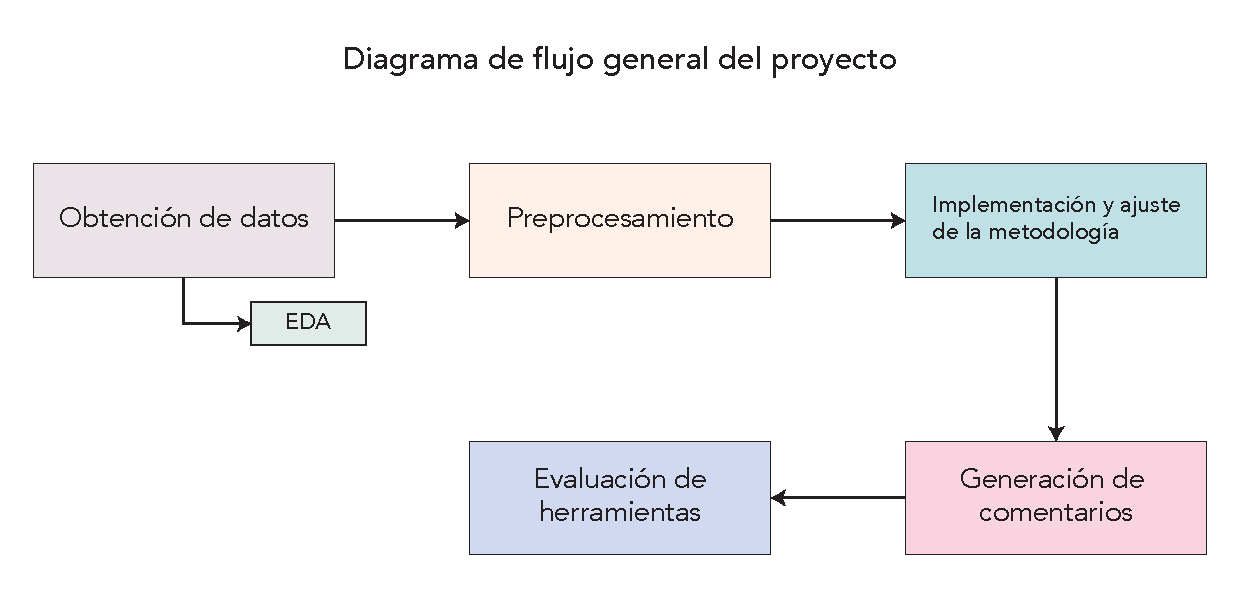
\includegraphics[width=.9\textwidth]{media/general.pdf}
	\caption{Diagrama de flujo general de todo el proyecto}
	\label{fig:general-diagram}
\end{figure}

En cada uno de los capítulos siguientes ahondaremos en cada uno de las fases, respectivamente, explicando en profundidad en qué consisten, cual es su entrada, su salida y su objetivo.

